
\begin{frame}
\centering
This presentation has approximately five
lines of math in it.
\\
This presentation has approximately 300
lines of code in it.
\\[2em]
All of the automation is written in python. \\
Consider your tools and their limitations.
\\[2em]
There are three examples in ascending order
of difficulty.  
\end{frame}

\begin{frame}
\tableofcontents
\end{frame}

\begin{Verbatim}[commandchars=\\\{\},numbers=left,numbersep=0.5em]
\PY{k+kn}{from} \PY{n+nn}{\PYZus{}\PYZus{}future\PYZus{}\PYZus{}} \PY{k+kn}{import} \PY{n}{print\PYZus{}function}

\PY{k+kn}{import} \PY{n+nn}{numpy} \PY{k+kn}{as} \PY{n+nn}{np}
\PY{k+kn}{import} \PY{n+nn}{os}
\PY{k+kn}{from} \PY{n+nn}{grid} \PY{k+kn}{import} \PY{n}{template}

\PY{n}{tex} \PY{o}{=} \PY{l+s}{r\PYZdq{}\PYZdq{}\PYZdq{}}
\PY{l+s}{\PYZbs{}}\PY{l+s}{begin\PYZob{}align\PYZcb{}}
\PY{l+s}{A\PYZus{}[=[i]=] \PYZam{} = }
\PY{l+s}{\PYZbs{}}\PY{l+s}{begin\PYZob{}pmatrix\PYZcb{}}
\PY{l+s}{\PYZbs{}}\PY{l+s}{input\PYZob{}../img/matrices/[=[i]=].tex\PYZcb{}}
\PY{l+s}{\PYZbs{}}\PY{l+s}{end\PYZob{}pmatrix\PYZcb{} }\PY{l+s}{\PYZbs{}}\PY{l+s}{\PYZbs{}}
\PY{l+s}{|A\PYZus{}[=[i]=]| \PYZam{} = [=[d]=] }\PY{l+s}{\PYZbs{}}\PY{l+s}{\PYZbs{}}
\PY{l+s}{A\PYZus{}[=[i]=]\PYZca{}\PYZob{}\PYZhy{}1\PYZcb{} \PYZam{} = }
\PY{l+s}{\PYZbs{}}\PY{l+s}{begin\PYZob{}pmatrix\PYZcb{}}
\PY{l+s}{\PYZbs{}}\PY{l+s}{input\PYZob{}../img/matrices/[=[i]=]i.tex\PYZcb{}}
\PY{l+s}{\PYZbs{}}\PY{l+s}{end\PYZob{}pmatrix\PYZcb{} }\PY{l+s}{\PYZbs{}}\PY{l+s}{\PYZbs{}}
\PY{l+s}{|A\PYZus{}[=[i]=]\PYZca{}\PYZob{}\PYZhy{}1\PYZcb{}| \PYZam{} = [=[di]=]}
\PY{l+s}{\PYZbs{}}\PY{l+s}{end\PYZob{}align\PYZcb{}}
\PY{l+s}{\PYZdq{}\PYZdq{}\PYZdq{}}

\PY{k}{def} \PY{n+nf}{doit}\PY{p}{(}\PY{n}{outdir}\PY{p}{)}\PY{p}{:}
  \PY{k}{for} \PY{n}{i} \PY{o+ow}{in} \PY{n+nb}{range}\PY{p}{(}\PY{l+m+mi}{5}\PY{p}{)}\PY{p}{:}
    \PY{n}{A} \PY{o}{=} \PY{n}{np}\PY{o}{.}\PY{n}{random}\PY{o}{.}\PY{n}{randn}\PY{p}{(}\PY{l+m+mi}{4}\PY{p}{,}\PY{l+m+mi}{4}\PY{p}{)}
    \PY{n}{np}\PY{o}{.}\PY{n}{savetxt}\PY{p}{(}
      \PY{n}{os}\PY{o}{.}\PY{n}{path}\PY{o}{.}\PY{n}{join}\PY{p}{(}\PY{n}{outdir}\PY{p}{,} \PY{l+s}{\PYZdq{}}\PY{l+s}{\PYZob{}\PYZcb{}.tex}\PY{l+s}{\PYZdq{}}\PY{o}{.}\PY{n}{format}\PY{p}{(}\PY{n}{i}\PY{p}{)}\PY{p}{)}\PY{p}{,}
      \PY{n}{A}\PY{p}{,}
      \PY{n}{fmt}\PY{o}{=}\PY{l+s}{\PYZdq{}}\PY{l+s+si}{\PYZpc{}5.3f}\PY{l+s}{\PYZdq{}}\PY{p}{,}
      \PY{n}{delimiter}\PY{o}{=}\PY{l+s}{\PYZdq{}}\PY{l+s}{ \PYZam{} }\PY{l+s}{\PYZdq{}}\PY{p}{,}
      \PY{n}{newline}\PY{o}{=}\PY{l+s}{\PYZdq{}}\PY{l+s}{ }\PY{l+s+se}{\PYZbs{}\PYZbs{}}\PY{l+s+se}{\PYZbs{}\PYZbs{}}\PY{l+s+se}{\PYZbs{}n}\PY{l+s}{\PYZdq{}}\PY{p}{,}
      \PY{p}{)}
    \PY{n}{Ai} \PY{o}{=} \PY{n}{np}\PY{o}{.}\PY{n}{linalg}\PY{o}{.}\PY{n}{inv}\PY{p}{(}\PY{n}{A}\PY{p}{)}
    \PY{n}{np}\PY{o}{.}\PY{n}{savetxt}\PY{p}{(}
      \PY{n}{os}\PY{o}{.}\PY{n}{path}\PY{o}{.}\PY{n}{join}\PY{p}{(}\PY{n}{outdir}\PY{p}{,} \PY{l+s}{\PYZdq{}}\PY{l+s}{\PYZob{}\PYZcb{}i.tex}\PY{l+s}{\PYZdq{}}\PY{o}{.}\PY{n}{format}\PY{p}{(}\PY{n}{i}\PY{p}{)}\PY{p}{)}\PY{p}{,}
      \PY{n}{Ai}\PY{p}{,}
      \PY{n}{fmt}\PY{o}{=}\PY{l+s}{\PYZdq{}}\PY{l+s+si}{\PYZpc{}5.3f}\PY{l+s}{\PYZdq{}}\PY{p}{,}
      \PY{n}{delimiter}\PY{o}{=}\PY{l+s}{\PYZdq{}}\PY{l+s}{ \PYZam{} }\PY{l+s}{\PYZdq{}}\PY{p}{,}
      \PY{n}{newline}\PY{o}{=}\PY{l+s}{\PYZdq{}}\PY{l+s}{ }\PY{l+s+se}{\PYZbs{}\PYZbs{}}\PY{l+s+se}{\PYZbs{}\PYZbs{}}\PY{l+s+se}{\PYZbs{}n}\PY{l+s}{\PYZdq{}}\PY{p}{,}
      \PY{p}{)}
    \PY{n}{d} \PY{o}{=} \PY{n}{np}\PY{o}{.}\PY{n}{linalg}\PY{o}{.}\PY{n}{det}\PY{p}{(}\PY{n}{A}\PY{p}{)}
    \PY{n}{di} \PY{o}{=} \PY{n}{np}\PY{o}{.}\PY{n}{linalg}\PY{o}{.}\PY{n}{det}\PY{p}{(}\PY{n}{Ai}\PY{p}{)}
    
    \PY{n}{fname} \PY{o}{=} \PY{l+s}{\PYZdq{}}\PY{l+s}{summary\PYZob{}\PYZcb{}.tex}\PY{l+s}{\PYZdq{}}\PY{o}{.}\PY{n}{format}\PY{p}{(}\PY{n}{i}\PY{p}{)}
    \PY{k}{with} \PY{n+nb}{open}\PY{p}{(}\PY{n}{os}\PY{o}{.}\PY{n}{path}\PY{o}{.}\PY{n}{join}\PY{p}{(}\PY{n}{outdir}\PY{p}{,}\PY{n}{fname}\PY{p}{)}\PY{p}{,}\PY{l+s}{\PYZdq{}}\PY{l+s}{w}\PY{l+s}{\PYZdq{}}\PY{p}{)} \PY{k}{as} \PY{n}{fout}\PY{p}{:}
      \PY{n}{fout}\PY{o}{.}\PY{n}{write}\PY{p}{(}\PY{n}{template}\PY{p}{(}\PY{n}{tex}\PY{p}{)}\PY{o}{.}\PY{n}{format}\PY{p}{(}
        \PY{n}{i}\PY{o}{=}\PY{n}{i}\PY{p}{,}
        \PY{n}{d}\PY{o}{=}\PY{l+s}{\PYZdq{}}\PY{l+s}{\PYZob{}:.3f\PYZcb{}}\PY{l+s}{\PYZdq{}}\PY{o}{.}\PY{n}{format}\PY{p}{(}\PY{n}{d}\PY{p}{)}\PY{p}{,}
        \PY{n}{di}\PY{o}{=}\PY{l+s}{\PYZdq{}}\PY{l+s}{\PYZob{}:.3f\PYZcb{}}\PY{l+s}{\PYZdq{}}\PY{o}{.}\PY{n}{format}\PY{p}{(}\PY{n}{di}\PY{p}{)}\PY{p}{,}
        \PY{p}{)}\PY{p}{)}

\PY{c}{\PYZsh{}\PYZdl{} simple\PYZus{}problem}
\PY{k}{def} \PY{n+nf}{simple\PYZus{}problem}\PY{p}{(}\PY{n}{outdir}\PY{p}{)}\PY{p}{:}
  \PY{n}{A} \PY{o}{=} \PY{n}{np}\PY{o}{.}\PY{n}{matrix}\PY{p}{(}\PY{p}{[}
    \PY{p}{[}\PY{l+m+mi}{3}\PY{p}{,} \PY{l+m+mi}{5}\PY{p}{,} \PY{l+m+mi}{2}\PY{p}{]}\PY{p}{,}
    \PY{p}{[}\PY{l+m+mi}{1}\PY{p}{,} \PY{l+m+mi}{6}\PY{p}{,} \PY{l+m+mi}{2}\PY{p}{]}\PY{p}{,}
    \PY{p}{[}\PY{l+m+mi}{1}\PY{p}{,} \PY{l+m+mi}{1}\PY{p}{,} \PY{l+m+mi}{1}\PY{p}{]}\PY{p}{,}
    \PY{p}{]}\PY{p}{)}
  \PY{n}{b} \PY{o}{=} \PY{n}{np}\PY{o}{.}\PY{n}{matrix}\PY{p}{(}\PY{p}{[}\PY{l+m+mi}{1}\PY{p}{,}\PY{l+m+mi}{2}\PY{p}{,}\PY{l+m+mi}{3}\PY{p}{]}\PY{p}{)}\PY{o}{.}\PY{n}{T}
  \PY{n}{x} \PY{o}{=} \PY{n}{np}\PY{o}{.}\PY{n}{linalg}\PY{o}{.}\PY{n}{solve}\PY{p}{(}\PY{n}{A}\PY{p}{,} \PY{n}{b}\PY{p}{)}
  
  \PY{n}{pairs} \PY{o}{=} \PY{p}{[}\PY{p}{(}\PY{n}{A}\PY{p}{,}\PY{l+s}{\PYZdq{}}\PY{l+s}{A}\PY{l+s}{\PYZdq{}}\PY{p}{)}\PY{p}{,} \PY{p}{(}\PY{n}{b}\PY{p}{,}\PY{l+s}{\PYZdq{}}\PY{l+s}{b}\PY{l+s}{\PYZdq{}}\PY{p}{)}\PY{p}{,} \PY{p}{(}\PY{n}{x}\PY{p}{,}\PY{l+s}{\PYZdq{}}\PY{l+s}{x}\PY{l+s}{\PYZdq{}}\PY{p}{)}\PY{p}{]}
  \PY{k}{for} \PY{n}{v}\PY{p}{,} \PY{n}{name} \PY{o+ow}{in} \PY{n}{pairs}\PY{p}{:}
    \PY{n}{np}\PY{o}{.}\PY{n}{savetxt}\PY{p}{(}
      \PY{n}{os}\PY{o}{.}\PY{n}{path}\PY{o}{.}\PY{n}{join}\PY{p}{(}\PY{n}{outdir}\PY{p}{,} \PY{l+s}{\PYZdq{}}\PY{l+s}{\PYZob{}\PYZcb{}.tex}\PY{l+s}{\PYZdq{}}\PY{o}{.}\PY{n}{format}\PY{p}{(}\PY{n}{name}\PY{p}{)}\PY{p}{)}\PY{p}{,}
      \PY{n}{v}\PY{p}{,}
      \PY{n}{fmt}\PY{o}{=}\PY{l+s}{\PYZdq{}}\PY{l+s+si}{\PYZpc{}5.3f}\PY{l+s}{\PYZdq{}}\PY{p}{,}
      \PY{n}{delimiter}\PY{o}{=}\PY{l+s}{\PYZdq{}}\PY{l+s}{ \PYZam{} }\PY{l+s}{\PYZdq{}}\PY{p}{,}     \PY{c}{\PYZsh{} These two lines }
      \PY{n}{newline}\PY{o}{=}\PY{l+s}{\PYZdq{}}\PY{l+s}{ }\PY{l+s+se}{\PYZbs{}\PYZbs{}}\PY{l+s+se}{\PYZbs{}\PYZbs{}}\PY{l+s+se}{\PYZbs{}n}\PY{l+s}{\PYZdq{}}\PY{p}{,}   \PY{c}{\PYZsh{} enable latex inputs.}
      \PY{p}{)}
\PY{c}{\PYZsh{}\PYZdl{}    }

\PY{k}{if} \PY{n}{\PYZus{}\PYZus{}name\PYZus{}\PYZus{}} \PY{o}{==} \PY{l+s}{\PYZdq{}}\PY{l+s}{\PYZus{}\PYZus{}main\PYZus{}\PYZus{}}\PY{l+s}{\PYZdq{}}\PY{p}{:}
  \PY{n}{doit}\PY{p}{(}\PY{l+s}{\PYZdq{}}\PY{l+s}{../img/matrices}\PY{l+s}{\PYZdq{}}\PY{p}{)}
  \PY{n}{simple\PYZus{}problem}\PY{p}{(}\PY{l+s}{\PYZdq{}}\PY{l+s}{../tex/pieces}\PY{l+s}{\PYZdq{}}\PY{p}{)}
\end{Verbatim}

\begin{Verbatim}[commandchars=\\\{\},numbers=left,numbersep=0.5em,firstnumber=9]
\PY{k}{def} \PY{n+nf}{fourier}\PY{p}{(}\PY{n}{freq}\PY{p}{,} \PY{n}{components}\PY{p}{,} \PY{n}{tlims}\PY{o}{=}\PY{p}{[}\PY{l+m+mi}{0}\PY{p}{,}\PY{l+m+mi}{1}\PY{p}{]}\PY{p}{)}\PY{p}{:}
  \PY{l+s+sd}{\PYZdq{}\PYZdq{}\PYZdq{}}
\PY{l+s+sd}{  freq is a number}
\PY{l+s+sd}{  components is a list of numbers}
\PY{l+s+sd}{  \PYZdq{}\PYZdq{}\PYZdq{}}
  \PY{n}{t} \PY{o}{=} \PY{n}{np}\PY{o}{.}\PY{n}{linspace}\PY{p}{(}\PY{o}{*}\PY{n}{tlims}\PY{p}{,} \PY{n}{num}\PY{o}{=}\PY{l+m+mi}{1000}\PY{p}{)}
  \PY{n}{y} \PY{o}{=} \PY{l+m+mi}{0}\PY{o}{*}\PY{n}{t}
  \PY{k}{for} \PY{n}{n} \PY{o+ow}{in} \PY{n}{components}\PY{p}{:}
    \PY{n}{y} \PY{o}{+}\PY{o}{=} \PY{l+m+mf}{1.0}\PY{o}{/}\PY{n}{n} \PY{o}{*} \PY{n}{np}\PY{o}{.}\PY{n}{sin}\PY{p}{(}\PY{l+m+mi}{2}\PY{o}{*}\PY{n}{np}\PY{o}{.}\PY{n}{pi}\PY{o}{*}\PY{p}{(}\PY{n}{freq}\PY{o}{*}\PY{n}{n}\PY{p}{)}\PY{o}{*}\PY{n}{t}\PY{p}{)}
  \PY{k}{return} \PY{n}{t}\PY{p}{,} \PY{n}{y}
\end{Verbatim}

\section{Code Snippets}
\begin{frame}
\tableofcontents[currentsection]
\end{frame}

%$ using_snippets
\subsection{Defining Latex Commands}
\begin{frame}
\frametitle{Using Snippets}
Sometimes, discussion revolves around code 
snippets.  We would like to include these 
snippets using a simple command.
% We want a snippet here!
\snippet{tex/using_snippets}
% Did it work?!?
This slide shows the latex source code to
generate this slide.  (Recursive logic...?)
\end{frame}
%$

\begin{frame}
\frametitle{Snippet Command}
\snippet{tex/beamer_snippets}
\end{frame}

\subsection{Pygments}
\begin{frame}
\frametitle{Pygmentize!}
Pygments colors any source code with a variety
of possible output formats.
\begin{center}
\begin{minipage}{.6\linewidth}
\noindent
{\bf pygmentize} -f latex -o output.tex input.tex \\
\noindent
{\bf pygmentize} -f html -o output.html input.tex
\end{minipage}
\end{center}
The following is an example of calling the 
command line function from within python.  
Three optional arguments are specified.
\snippet{py/pygmentize}
\end{frame}

% pygmentize -f tex -o verbatim_table_colored.tex verbatim_table_excerpt.tex 
\begin{frame}[fragile]
\frametitle{Typical Source Code with Snippet}
\begin{minipage}{.35\linewidth}
We want to pull out the snippet of code
surrounded by ``{\bf \%\$}'', which we have 
defined to be the start and stop markers of
{\bf snippets}.
\\[1em]
The code on the right is an excerpt from Slide
\pageref{slide/matricesandtables}, where we 
showed how to input a matrix from a file into
a table.
\end{minipage}
\hfill
\begin{minipage}{.6\linewidth}
\begin{small}
\begin{Verbatim}[commandchars=\\\{\}]
\PY{k}{\PYZbs{}end}\PY{n+nb}{\PYZob{}}center\PY{n+nb}{\PYZcb{}}
The contents of \PY{k}{\PYZbs{}verb}|A.tex| can be 
made into a table. \PY{k}{\PYZbs{}\PYZbs{}}\PY{n+na}{[1em]}
\PY{k}{\PYZbs{}begin}\PY{n+nb}{\PYZob{}}minipage\PY{n+nb}{\PYZcb{}}\PY{n+nb}{\PYZob{}}.45\PY{k}{\PYZbs{}linewidth}\PY{n+nb}{\PYZcb{}}
\PY{k}{\PYZbs{}centering}
\PY{c}{\PYZpc{}\PYZdl{} simple\PYZus{}table}
\PY{k}{\PYZbs{}begin}\PY{n+nb}{\PYZob{}}tabular\PY{n+nb}{\PYZcb{}}\PY{n+nb}{\PYZob{}}c c c\PY{n+nb}{\PYZcb{}}
\PY{l+s}{\PYZdl{}}\PY{n+nb}{C}\PY{n+nb}{\PYZus{}}\PY{l+m}{1}\PY{l+s}{\PYZdl{}} \PY{n+nb}{\PYZam{}} \PY{l+s}{\PYZdl{}}\PY{n+nb}{C}\PY{n+nb}{\PYZus{}}\PY{l+m}{2}\PY{l+s}{\PYZdl{}} \PY{n+nb}{\PYZam{}} \PY{l+s}{\PYZdl{}}\PY{n+nb}{C}\PY{n+nb}{\PYZus{}}\PY{l+m}{3}\PY{l+s}{\PYZdl{}} \PY{k}{\PYZbs{}\PYZbs{}}
\PY{k}{\PYZbs{}midrule}
\PY{k}{\PYZbs{}input}\PY{n+nb}{\PYZob{}}pieces/A.tex\PY{n+nb}{\PYZcb{}}
\PY{k}{\PYZbs{}end}\PY{n+nb}{\PYZob{}}tabular\PY{n+nb}{\PYZcb{}}
\PY{c}{\PYZpc{}\PYZdl{}}
\PY{k}{\PYZbs{}end}\PY{n+nb}{\PYZob{}}minipage\PY{n+nb}{\PYZcb{}}
\PY{k}{\PYZbs{}begin}\PY{n+nb}{\PYZob{}}minipage\PY{n+nb}{\PYZcb{}}\PY{n+nb}{\PYZob{}}.45\PY{k}{\PYZbs{}linewidth}\PY{n+nb}{\PYZcb{}}
\end{Verbatim}

\end{small}
\end{minipage}
\end{frame}

\subsection{Python Solution}
\begin{frame}[fragile]
\frametitle{Define Patterns to Match}
Each file is text.  Process each file 
sequentially line by line.
\\[1em]
Look for comments in the code that
that have a snippet name preceded by a 
specific pattern.
\begin{center}
{\bf \%\$ snippet\_name}
\end{center}
Different languages use different comment
delimiters, so define a pattern
for each language of interest.
\snippet{py/define_matches}
(Python dictionary!  
The variable \verb|exts[".m"]|
contains the text \verb|"%$"|.)
\end{frame}

\begin{frame}
\frametitle{Identifying Snippets}
\snippet{py/snipdef}
\end{frame}

\begin{frame}
\frametitle{Collect Lines for Each Snippet}
\snippet{py/collect_lines}
\end{frame} 

\begin{frame}
\frametitle{Write Lines of Each Snippet}
\snippet{py/write_snippets}
\end{frame}

%$ snippet_example
% Here's this slide's source, an
% example of using snippets!
\begin{frame}
\frametitle{Call Pygmentize and Use Snippets}
\snippet{py/pygmentize}
\snippet{tex/snippet_example}
\end{frame}
%$

\section*{Discussion}
\begin{frame}
\frametitle{Nothing Left? :D}
\tableofcontents[currentsection]
\end{frame}

\begin{frame}
\frametitle{Parsing Logs}
\begin{minipage}{.4\linewidth}
Parsing through source code to find keywords
is similar to parsing through log files to
find keywords.
\\[1em]
Parse logs to generate tabular data in order
to avoid needing to make layout decisions in
advance.
\\[1em]
Having the power to change your mind 
is {\bf valuable}.
\end{minipage}
\hfill
\begin{minipage}{.55\linewidth}
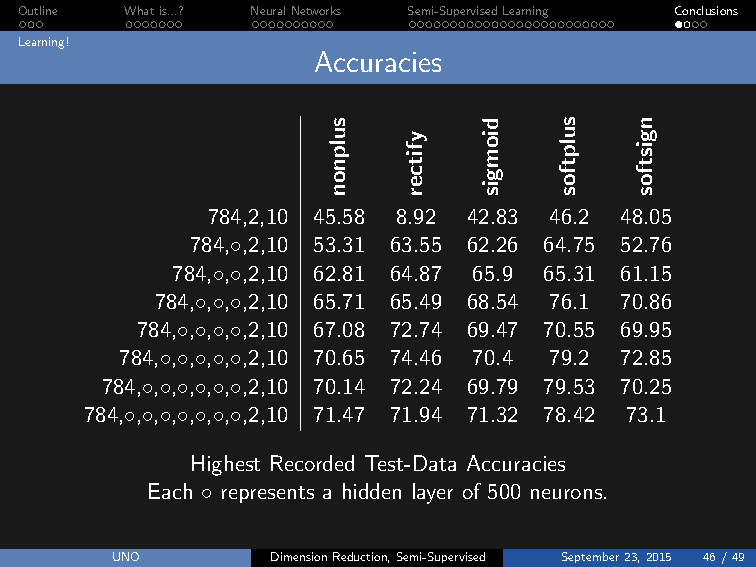
\includegraphics[width=\linewidth]{%
../img/Table_Only_2015_09_23_learning.pdf}
\end{minipage}
\end{frame}

\begin{frame}
\frametitle{Discussion}
How often do EE students/professors need
to include source code?
What about the {\bf listings} package?
\\[1em]
How severe is the penalty of making a mistake
or having inconsistent documents due to
copying and pasting code/figures/tables?
\\[1em]
Reproducible Research!
\\[1em]
Uses of Latex outside of papers/presentations?
\\[1em]
Bonus!  Check out those partially-highlighted outlines.
\snippet{tex/currentsection}
\end{frame}

\begin{frame}
\frametitle{Directory Listing of this Presentation}
% tree --charset=ascii ../tex ../code ../img > pieces/tree.txt
\vspace{-1em}
\hfill 
\begin{minipage}{.9\linewidth}
\begin{multicols}{3}
\begin{Tiny}
\verbatiminput{pieces/tree.txt}
\end{Tiny}
\end{multicols}
\end{minipage}
\hfill
\end{frame}
